\documentclass[journal]{IEEEtran}
\usepackage{graphicx}
\usepackage{amsmath}
\usepackage{hyperref}
\usepackage{float}
\usepackage{subcaption}
\usepackage{booktabs}
\usepackage{pgfplotstable}
\usepackage{qrcode}

\pgfplotsset{compat=1.18}

\begin{document}

% Title Section
\title{Magnetic Resonance in Coupled Thomson Oscillators}
\author{IBRAHIM H.I. ABUSHAWISH \\
Istanbul University, Department of Physics \\
Instructor: Res. Asst. Dilan AKHAN  \\
Experiment Date: 09.12.2024, Report Submission Date: 16.12.2024 \\
Course \& Section Number: PHYS2305}

\maketitle


\begin{abstract}
This report presents a comprehensive analysis of magnetic resonance in coupled Thomson oscillators. It provides a detailed theoretical overview, experimental procedures, data analysis, and discussion of key findings. The analysis is supported by calculations and graphical visualizations. Key conclusions are highlighted, particularly on the resonance frequency shift under varying capacitor settings.
\end{abstract}


\begin{IEEEkeywords}
Magnetic Resonance, Thomson Oscillator, Electromagnetic Coupling, Frequency Analysis
\end{IEEEkeywords}


% Introduction
\section{Introduction}
This section introduces the concept of magnetic resonance in coupled Thomson oscillators. The primary aim is to investigate the conditions under which two electromagnetically coupled circuits achieve resonance. This phenomenon is critical in understanding electromagnetic transmission and energy transfer in coupled oscillatory systems.
% Theoretical Background
\section{Theoretical Background}
Theoretical background was taken mostly from \cite{lab_manual}.

\textbf{1. Vibrational Motion:}
Vibrational motion occurs when a system oscillates around its equilibrium due to an external force. The time for one complete oscillation is called the period \(\tau\), while the number of oscillations per second is the frequency \(f\). The two are related by:
\begin{equation}
    f \cdot \tau = 1
\end{equation}
The maximum displacement during oscillation is the amplitude. If oscillations lose energy over time, the vibration is damped; if not, it is undamped.

\textbf{2. Resonance:}
When a system is subjected to a periodic force with a frequency matching its natural frequency, its amplitude reaches a maximum—a condition called resonance. This occurs at the resonance frequency \(f_r\). The period \(\tau\) and frequency \(f\) have the units:
\begin{equation}
    [\tau] = s, \quad [f] = s^{-1} = Hertz (Hz)
\end{equation}

\textbf{3. Thomson Vibration Circuit:}
A Thomson circuit consists of a capacitor \(C\) and an inductor \(L\) connected together. When the charged capacitor discharges, current flows through the inductor, creating a magnetic field. As the capacitor discharges, its charge decreases, while the current in the inductor increases. This process repeats, resulting in oscillations. The period of oscillation \(\tau\) is:
\begin{equation}
    \tau = 2\pi \sqrt{LC}
\end{equation}
where \(L\) and \(C\) are the inductance (measured in Henrys) and capacitance (measured in Farads), respectively.

\textbf{4. Magnetic Coupling:}
When two Thomson circuits are placed close to each other, magnetic coupling occurs. The magnetic field of one circuit induces an electromotive force (emf) in the other. If the oscillation frequencies of the two circuits match, resonance occurs, maximizing the energy transfer between the circuits.

The self-vibration frequencies of the two coupled circuits are:
\begin{equation}
    f_1 = \frac{1}{2\pi \sqrt{L_1 C_1}}, \quad f_2 = \frac{1}{2\pi \sqrt{L_2 C_2}}
\end{equation}
When \(f_1 = f_2\), maximum current flows in the second circuit. This resonance condition is mathematically represented as:
\begin{equation}
    L_1 C_1 = L_2 C_2
\end{equation}
In this scenario, the first circuit acts as a transmitter, and the second as a receiver. By adjusting the capacitance or inductance, the frequencies can be matched to achieve resonance.

% \begin{figure}[H]
%    \centering
%    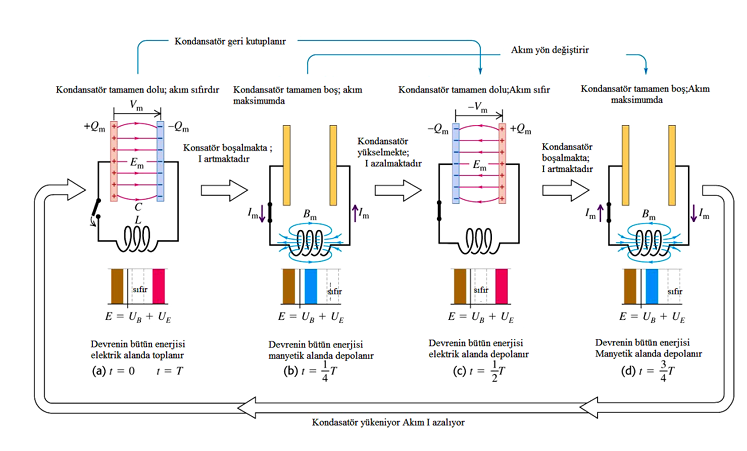
\includegraphics[width=0.9\linewidth]{IMAGES/demonstration_diagram.png}
%    \caption{Demonstration of Energy Oscillations in Coupled Circuits.}
%    \label{fig:demonstration_diagram}
%\end{figure}

\section{Experimental Setup}
The experimental setup Figs.~\ref{fig:exp_setup} and ~\ref{fig:exp_diagram} includes a Hartley oscillator circuit using a TIP 15A transistor as the transmitter and a coupled receiver circuit. The setup also incorporates variable capacitors and a microammeter to measure resonance response. The primary components are:
\begin{itemize}
    \item Transmitter: Hartley oscillator with adjustable capacitance.
    \item Receiver: Coupled Thomson oscillator with a microammeter for current measurement.
    \item Variable capacitors \( C_1 \) and \( C_2 \) for tuning the resonance condition.
\end{itemize}

\begin{figure}[H]
    \centering
    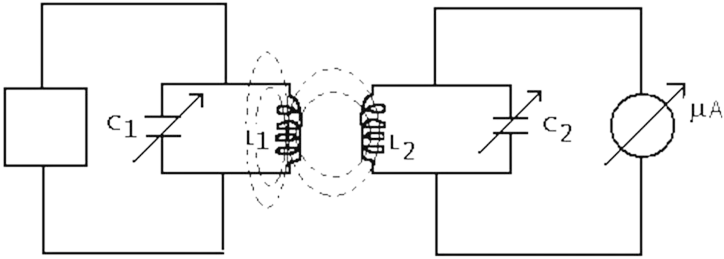
\includegraphics[width=0.8\linewidth]{IMAGES/Experimental_diagram.png}
    \caption{Diagrammatic Representation of Experimental Setup}
    \label{fig:exp_diagram}
\end{figure}

\begin{figure}[H]
    \centering
    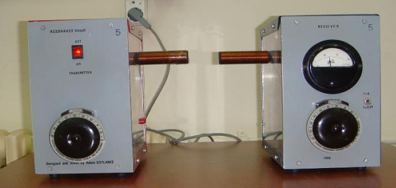
\includegraphics[width=0.8\linewidth]{IMAGES/Experimental_setup.png}
    \caption{Physical Experimental Setup with Transmitter and Receiver}
    \label{fig:exp_setup}
\end{figure}

\section{Methodology}
The experiment begins by activating the transmitter and aligning the receiver to achieve magnetic coupling. The capacitance \(C_1\) of the transmitter is varied, and the corresponding receiver current is measured. This process is repeated for different capacitance values to observe changes in current as the system approaches resonance.

Next, the capacitance \(C_2\) of the receiver is adjusted to match the self-vibration frequencies of both circuits. As the frequencies align, the current in the receiver peaks at resonance. Measurements of capacitance and current are recorded for further analysis.

The effect of resistance in the receiver circuit is also investigated. Higher resistance lowers the peak current and broadens the resonance curve, indicating the damping effect of resistance on the system. The collected data is used to analyze the relationship between capacitance, resistance, and resonance behavior in coupled Thomson oscillators.


% Results
\section{Results}
The following data, figures and calculations can also be found in the GitHub repository \cite{github} in \texttt{DATA/} and \texttt{output\_plots/}, under \texttt{6th\_Experiment\_Magnetic\_Resonance/}.

The results of the experiment are tabulated as follows:

\begin{table}[H]
    \centering
    
    \pgfplotstabletypeset[col sep=comma, header=true]{DATA/C_vs_I_r_0.csv}

    \caption{Current Intensity as a Function of Capacitance \( C_2 \) (\( R = 0 \))}
    \label{tab:c2_r0}
\end{table}

\begin{table}[H]
    \centering
    \pgfplotstabletypeset[col sep=comma, header=true]{DATA/C_vs_I_r_22.csv}
    \caption{Current Intensity as a Function of Capacitance \( C_2 \) (\( R = 2.2k\Omega \))}
    \label{tab:c2_r22}
\end{table}

The analysis reveals the conditions under which resonance is achieved. The maximum current flow occurs when the self-vibration frequencies of the two coupled circuits match, as indicated by the peak in the \( I = f(C_2) \) curve. The effects of varying resistance \( R \) are also discussed. When \( R = 2.2k\Omega \), the resonance peak shifts, highlighting the influence of resistance on resonance behavior.

\begin{figure}[H]
    \centering
    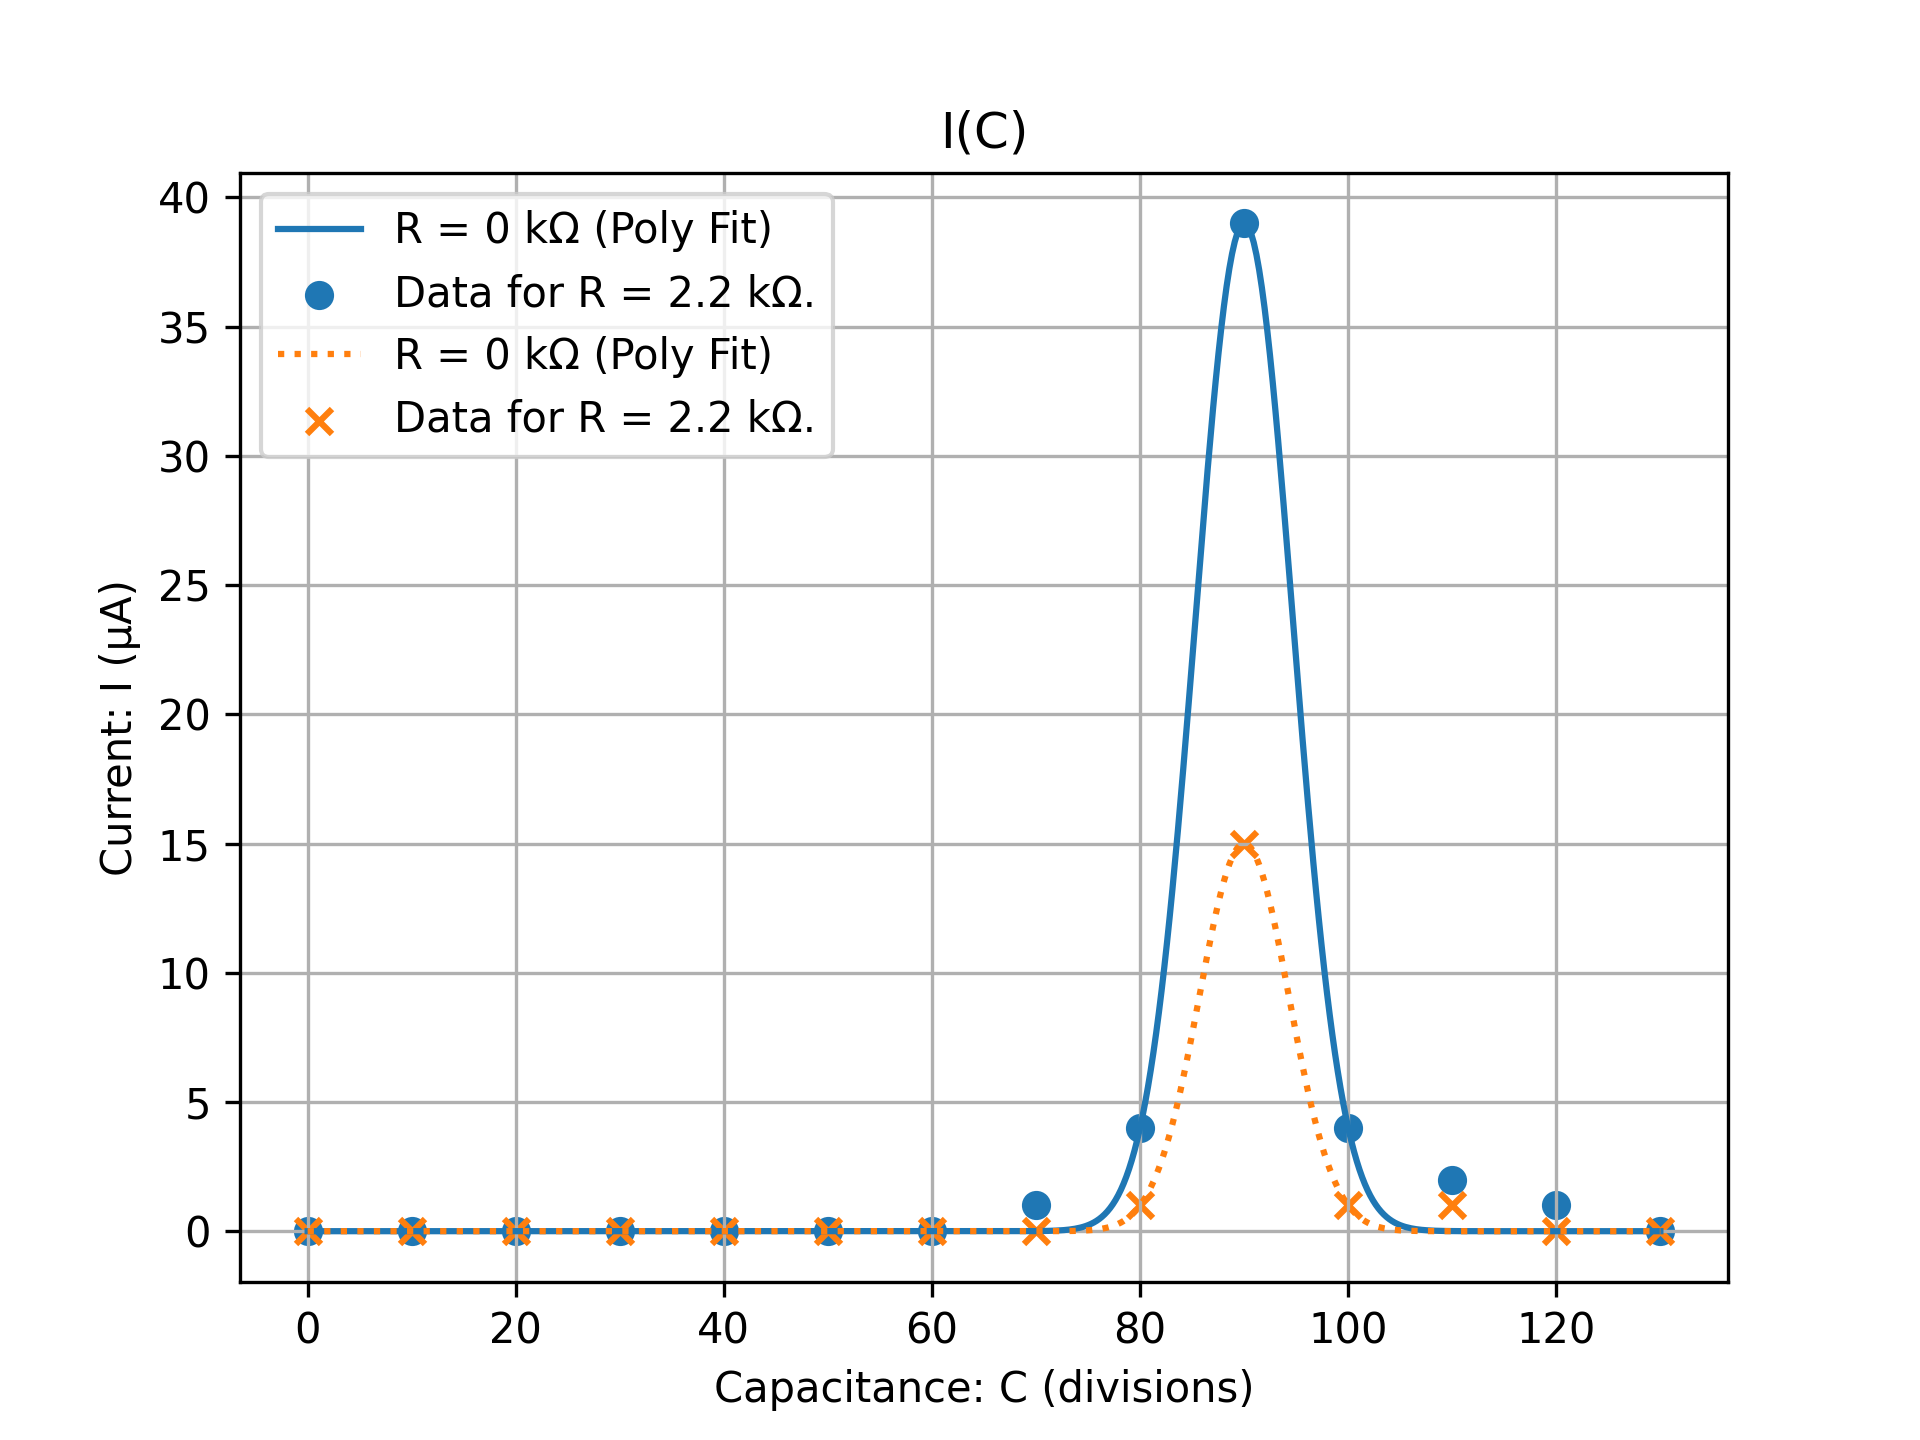
\includegraphics[width=\linewidth]{output_plots/current_vs_Capacitance.png}
    \caption{Current vs. Capacitance for Different Resistances}
    \label{fig:current_vs_capacitance}
\end{figure}

% Discussion
\section{Discussion}
The results from the experiment demonstrate the effect of capacitance and resistance on resonance in coupled Thomson oscillators. As observed in the graph, the resonance condition occurs when the capacitance values are adjusted such that the self-vibration frequencies of the transmitter and receiver circuits align. At this point, the current in the receiver circuit reaches its maximum value, indicating efficient energy transfer between the two circuits.

When the resistance \( R \) is set to \( 0 \, \text{k}\Omega \), the resonance curve is sharp and the peak current is significantly higher. This behavior aligns with theoretical predictions, as minimal resistance reduces energy losses in the system, allowing for stronger resonance. On the other hand, when \( R = 2.2 \, \text{k}\Omega \), the peak current is notably lower, and the resonance curve is broader. This indicates increased damping due to higher resistance, which causes energy losses and reduces the efficiency of energy transfer. The broadening of the curve also suggests that the system is less sensitive to changes in capacitance near the resonance condition.

The symmetry of the resonance curves confirms that the oscillations behave predictably around the resonance point. The results illustrate how resistance influences the sharpness and amplitude of resonance in coupled oscillatory systems.

% Conclusion
\section{Conclusion}
This experiment highlights the principles of resonance in coupled Thomson oscillators and demonstrates the effect of resistance on resonance behavior. The resonance condition, where maximum current occurs in the receiver circuit, is achieved by aligning the self-vibration frequencies of the transmitter and receiver circuits through capacitance adjustment. Lower resistance results in sharper and higher resonance peaks, while higher resistance reduces the peak current and broadens the resonance curve due to damping effects.

The experimental results confirm the theoretical relationships between capacitance, resistance, and resonance in oscillatory systems. Future studies could explore additional factors influencing resonance, such as variations in the inductance or the spatial alignment of the circuits to further understand the energy transfer mechanisms in coupled oscillators.

\section{Additional Resources}
For detailed information, including the Lab Manual, source code, and related experiments, visit the GitHub repository provided below or scan the QR code in Fig.~\ref{fig:qr_code}.

\begin{figure}[H]
    
    \centering
    \begin{minipage}{0.15\textwidth}
        \centering
        \qrcode[height=2cm]{https://github.com/ibeuler/LAB-Reports}
    \end{minipage}%
    \begin{minipage}{0.2\textwidth}
        \raggedright
        \caption{Access the GitHub repository for the lab manual, source code, and related experiments: \href{https://github.com/ibeuler/LAB-Reports}{\url{https://github.com/ibeuler/LAB-Reports}}.}
        \label{fig:qr_code}
    \end{minipage}
\end{figure}

\begin{thebibliography}{9}
\bibitem{lab_manual}
    ISTANBUL UNIVERSITY, \textit{Physics Laboratory II Experiment Book: Electricity and Magnetism}, Department of Physics, 2024.

\bibitem{github}
    \textit{Source code and additional experiments are available in the GitHub repository.} \url{https://github.com/ibeuler/LAB-Reports}
\end{thebibliography}

\end{document}
